\documentclass[a4paper, 14pt]{extarticle}
\usepackage[margin=1in]{geometry}
\usepackage{amsfonts, amsmath, amssymb, amsthm}
\usepackage[none]{hyphenat}
\usepackage{fancyhdr} %create a custom header and footer
\usepackage[utf8]{inputenc}
\usepackage[english, main=ukrainian]{babel}
\usepackage{pgfplots}
\usepgfplotslibrary{fillbetween}
\usepackage{tikz}
\usepackage{graphicx}
\usepackage{caption}
\usepackage{float}
\usepackage{physics}
\usepackage[unicode]{hyperref}
\usepgfplotslibrary{polar}
\usepackage{ifthen}
\usetikzlibrary{spy}
\usepackage{bbm}


\fancyhead{}
\fancyfoot{}
\parindent 0ex
\def\huge{\displaystyle}
\def\rightproof{$\boxed{\Rightarrow}$ }
\def\leftproof{$\boxed{\Leftarrow}$ }

\usepackage{pdfpages}

\newtheoremstyle{theoremdd}% name of the style to be used
  {\topsep}% measure of space to leave above the theorem. E.g.: 3pt
  {\topsep}% measure of space to leave below the theorem. E.g.: 3pt
  {\normalfont}% name of font to use in the body of the theorem
  {0pt}% measure of space to indent
  {\bfseries}% name of head font
  {}% punctuation between head and body
  { }% space after theorem head; " " = normal interword space
  {\thmname{#1}\thmnumber{ #2}\textnormal{\thmnote{ \textbf{#3}\\}}}

\theoremstyle{theoremdd}
\newtheorem{theorem}{Theorem}[subsection]
  
\theoremstyle{theoremdd}
\newtheorem{definition}[theorem]{Definition}

\theoremstyle{theoremdd}
\newtheorem{samedef}[theorem]{Definition}

\theoremstyle{theoremdd}
\newtheorem{example}[theorem]{Example}

\theoremstyle{theoremdd}
\newtheorem{proposition}[theorem]{Proposition}

\theoremstyle{theoremdd}
\newtheorem{remark}[theorem]{Remark}

\theoremstyle{theoremdd}
\newtheorem{lemma}[theorem]{Lemma}

\theoremstyle{theoremdd}
\newtheorem{corollary}[theorem]{Corollary}

\newenvironment{pf}{\vspace*{-3mm} \textbf{Proof. \\}}{$\blacksquare$}
\newenvironment{pfMI}{\vspace*{-3mm} \textbf{Proof MI. \\}}{$\blacksquare$}
\newenvironment{pfNoTh}{\textbf{Proof. \\}}{$\blacksquare$}

%delete

\begin{document}
\tableofcontents
\newpage

\section{Алгебра висловлень}
\subsection{Основа}
\begin{definition}
\textbf{Висловленням} називають речення, в якому можна визначити правдивість (true) або неправдивість (false) в даному контексті\\
Позначення: $A,B,\dots$ - їх ще 
називають \textbf{пропозиційними літерами}
\bigskip
\\
Якщо $A$ - true, то позначимо це $|A| = 1$\\
Якщо $A$ - false, то позначимо це $|A| = 0$\\
\end{definition}

\begin{example} Ось пару прикладів висловлень\\
$A = $ число 4 ділиться на 2. $|A|=1$\\
$B = $ число 4 - просте число. $|B|=0$
\bigskip
\\
Речення - число 4 дуже красиве - вже не є висловленням, тому що складно визначити правдивість або неправдивість
\end{example}

\subsubsection*{Основні операції}
\begin{definition}
Задані висловлення $A,B$\\
\textbf{Диз'юнкцією} називають висловлення $A \vee B$, що є true лише тоді, коли висловлення $A$ або $B$ - true\\
\textbf{Кон'юнкцією} називають висловлення $A \wedge B$, що є true лише тоді, коли висловлення $A$ та $B$ - true\\
\textbf{Запеченням} називають висловлення $\neg A$, що є true лише тоді, коли висловлення $A$ - false
\end{definition}

\begin{example} Із попереднього прикладу ми маємо, що\\
$A \vee B =$ число 4 ділиться на 2 або число 4 - просте число \hspace{0.5cm} $|A \vee B| = 1$\\
$A \wedge B = $ число 4 ділиться на 2 та число 4 - просте число \hspace{0.6cm} $|A \wedge B| = 0$\\
$\neg A =$ число 4 не просте число \hspace{6.4cm} $|\neg A| = 1$
\end{example}

\subsubsection*{Додаткові операції}
\begin{definition}
Задані висловлення $A,B$\\
\textbf{Імплікацією} називають висловлення $A \rightarrow B$, що є true лише тоді, коли з правдивості $A$ випливає правдивість $B$\\
Через основні операції: $A \rightarrow B = \neg A \vee B$
\bigskip \\
\textbf{Еквіваленцією} називають висловлення $A \leftrightarrow B$, що є true лише тоді, коли $A,B$ одночасно true або false\\
Через основні операції: $A \leftrightarrow B = (A \rightarrow B) \wedge (B \rightarrow A)$
\bigskip \\
\textbf{Сумою за модулем 2} називають висловлення $A \oplus B$, що є true лише тоді, коли лише один з висловлень $A$ або $B$ - true\\
Через основні операції: $A \oplus B = \neg(A \leftrightarrow B)$
\end{definition}

\begin{example} Задамо висловлення\\
$A = $ звук працює, $|A| = 1$ \hspace{0.5cm} $B = $ я чую, $|B| = 1$\\
$A \rightarrow B =$ якщо звук працює, то я чую \hspace{3.3cm} $|A \rightarrow B| = 1$\\
$A \leftrightarrow B =$ звук працює лише тоді, коли я чую \hspace{1.7cm} $|A \leftrightarrow B| = 1$\\
$A \oplus B =$ або лише звук працює, або лише я чую \hspace{1cm} $|A \oplus B| = 0$
\end{example}

\begin{definition}
\textbf{Формулою алгебри висловлень} будемо називати одним з двох пунктів\\
- пропозиційну літеру\\
- якщо $\mathcal{A}, \mathcal{B}$ формули, то $\mathcal{A} \vee \mathcal{B}$, $\mathcal{A} \wedge \mathcal{B}$, $\neg \mathcal{A}$ формули
\end{definition}

\subsection{Інтерпретація формул алгебри висловлень}
\begin{definition}
\textbf{Інтерпретацією} формули алгебри висловлень нази-\\вають зіставлення кожній пропозиційній літері значення $1$ (true) або $0$ (false)\\
Множину всіх інтерпретацій заданої формули зводиться в \textbf{таблицю правдивості}
\end{definition}

\begin{example}
Нехай задана формула $\mathcal{A} = A_1 \vee \neg A_2$. Внизу буде записана таблица правдивості
\begin{center}
\begin{tabular}{ |c|c|c| } 
 \hline
 $A_1$ & $A_2$ & $\mathcal{A}$ \\
 \hline
 $0$ & $0$ & $1$ \\ 
 $0$ & $1$ & $0$ \\ 
 $1$ & $0$ & $1$ \\
 $1$ & $1$ & $1$ \\ 
 \hline
\end{tabular}
\end{center}
Кожний рядок таблиці правдивості - це одна інтерпретація
\end{example}

\begin{example}
Задані висловлення $A,B$. Розпишемо таблиці правдивості для визначених операції вище
\begin{center}
\begin{tabular}{ |c|c|c|c|c|c|c| } 
 \hline
 $A$ & $B$ & $A \vee B$ & $A \wedge B$ & $A \rightarrow B$ & $A \leftrightarrow B$ & $A \oplus B$ \\
 \hline
 $0$ & $0$ & $0$ & $0$ & $1$ & $1$ & $0$ \\ 
 $0$ & $1$ & $1$ & $0$ & $1$ & $0$ & $1$ \\ 
 $1$ & $0$ & $1$ & $0$ & $0$ & $0$ & $1$ \\
 $1$ & $1$ & $1$ & $1$ & $1$ & $1$ & $0$ \\ 
 \hline
\end{tabular}
\end{center}
\end{example}

\begin{remark}
Зупинимось тут ще раз на імплікації. Нехай будуть такі висловлення\\
$A =$ босс сказав "працюй" ($|A| = 1$) або "роби, що хочеш" ($|A| = 0$)\\
$B = $ працівник йде працювати $(|B| = 1)$ або ледарить $(|B| = 0)$\\
А тепер подивимось на $A \rightarrow B$ зверху вниз\\
Якщо босс сказав "працюй", то працівник йде працювати - true\\
Якщо босс сказав "працюй", то працівник ледарить - false\\
Якщо босс сказав "роби, що хочеш", то працівник йде працювати - true\\
Якщо босс сказав "роби, що хочеш", то працівник ледарить - true\\
Останні два описують істину, тому що босс сказав те, що після цього можна робити що завгодно і він не оскаржить це \\
А тепер подивимось на $\neg A \vee B$\\
Або босс сказав "роби, що хочеш", або працівник йде працювати\\
Саме тому виявляється, що $A \rightarrow B = \neg A \vee B$
\bigskip \\
Звідки взялись інші формули, має бути зрозуміло
\end{remark}

\begin{remark}
Інколи для $A \rightarrow B$ кажуть так:\\
$B$ - необхідна умова для $A$ \hspace{0.5cm} $A$ - достатня умова для $B$\\
Щоб працівник пішов працювати, необхідно, щоб босс сказав йти працювти\\
Якщо босс скаже йти працювати, цього буде достатньо, щоб працівник пішов
\end{remark}

\begin{definition}
Формули $\mathcal{A}_1, \mathcal{A}_2$ називають \textbf{логічно еквівалентними}, якщо на кожній інтерпретації вони набувають однакових значенья\\
Позначення: $\mathcal{A}_1 = \mathcal{A}_2$ або $\mathcal{A}_1 \Leftrightarrow \mathcal{A}_2$
\end{definition}

\begin{example}
$A \vee B = B \vee A$ \hspace{1cm} $A \wedge B = B \wedge A$
\end{example}

\begin{definition}
Формулу $\mathcal{A}$ називають \textbf{тавтологією}, коли вона набуває значення $1$ на всіх інтерпретаціях\\
Позначення: $\mathcal{A} = 1$\\
Формулу $\mathcal{A}$ називають \textbf{суперечністю}, коли вона набуває значення $0$ на всіх інтерпретаціях\\
Позначення: $\mathcal{A} = 0$\\
Формулу $\mathcal{A}$ називають \textbf{таку, що виконується}, коли вона набуває значення $1$ хоча б на одній інтерпретації\\
\end{definition}

\begin{example}
$A \vee \neg A = 1$ \hspace{1cm} $A \wedge \neg A = 0$\\
Перша - тавтологія, бо всюди формула приймає true\\
Друга - суперечність, бо всюди формула приймає false
\end{example}

\subsection{Основні тотожності}
Задані формули алгебри висловлень $A,B,C$. Справедливі такі закони\\
1. Комутативність\\
$A \vee B = B \vee A$ \hspace{5cm} $A \wedge B = B \wedge A$\\
2. Дистрибутивність\\
$A \vee (B \wedge C) = (A \vee B) \wedge (A \vee C)$ \hspace{1cm} $A \wedge (B \vee C) = (A \wedge B) \vee (A \wedge C)$\\
3. Нейтральність\\
$A \vee 0 = A$ \hspace{6cm} $A \wedge 1 = A$\\
4. Доповненість\\
$A \vee \neg A = 1$ \hspace{5.6cm} $A \wedge \neg A = 0$\\
Всі вони доводяться за побудовою таблиць правдивостей. Решта виводяться та доводяться безпосередньо через ці тотожності
\bigskip \\
5. Універсальні межі\\
$A \vee 1 = 1$ \hspace{6cm} $A \wedge 0 = 0$\\
6. Абсорбція\\
$A \vee (A \wedge B) = A$ \hspace{4.4cm} $A \wedge (A \vee B) = A$\\
7. Ідемпотентність\\
$A \vee A = A$ \hspace{5.7cm} $A \wedge A = A$\\
8. Асоціативність\\
$A \vee (B \vee C) = (A \vee B) \vee C$ \hspace{2cm} $A \wedge (B \wedge C) = (A \wedge B) \wedge C$\\
9. Інвольвютивність\\
$\neg (\neg A) = A$\\
10. Правило де Моргана\\
$\neg(A \vee B) = \neg A \wedge \neg B$ \hspace{3cm} $\neg(A \wedge B) = \neg A \vee \neg B$
\bigskip
\\
\begin{pfNoTh}
Ми будемо доводити лише лівий стовпчик правил. Права аналогічна\\
5. $A \vee 1 = (A \vee 1) \vee 0 = (A \vee 1) \vee (A \wedge \neg A) = A \vee (1 \wedge \neg A) = A \vee \neg A = 1$
\bigskip \\
6. $A \vee (A \wedge B) = (A \wedge 1) \vee (A \wedge B) = A \wedge (1 \vee B) = A \wedge 1 = A$
\bigskip \\
7. $A \vee A = (A \vee A) \wedge 1 = (A \vee A) \wedge (A \vee \neg A) = A \vee (A \wedge \neg A) = A \vee 0 = A$
\bigskip \\
Решта три доводяться за допомогою такої леми
\begin{lemma}
Задано $D$ - формула алгебри висловлювань. Відомо, що\\
$X \wedge D = Y \wedge D$ \hspace{1cm} $X \wedge \neg D = Y \wedge \neg D$\\
Тоді $X=Y$
\end{lemma}
\begin{pf}
З одного боку,\\
$(X \wedge D) \vee (X \wedge \neg D) = X \wedge (D \vee \neg D) = X$\\
З іншого боку,\\
$(X \wedge D) \vee (X \wedge \neg D) = (Y \wedge D) \vee (Y \wedge \neg D) = Y \wedge (D \vee \neg D) = Y$\\
Отже, $X=Y$
\end{pf}
\bigskip \\
Продемонструю використання цієї леми лише на інвольвютивності (TODO)
\end{pfNoTh}

\subsection{Дуальність, узагальнене правило де Моргана}
\begin{definition}
Формула $\mathcal{A}^*$ називається \textbf{дуальною до} $\mathcal{A}$, коли вона є формулою $\mathcal{A}$, в якої\\
- $\vee$ замінюються на $\wedge$ або/та навпаки\\
- $0$ замінюються на $1$ або/та навпаки
\end{definition}

\begin{example}
$(A \vee \neg B \vee 0)^* = A \wedge \neg B \wedge 1$
\end{example}
Зрозуміло, що $\mathcal{A}^{**} = \mathcal{A}$

\begin{proposition}
Задано $\mathcal{A} = \mathcal{B}$. Тоді $\mathcal{A}^* = \mathcal{B}^*$
\end{proposition}

\begin{pf}
Коли $\mathcal{A} = \mathcal{B}$, то ліва частина перетворюється в праву частину шляхом використанням основних тотожностей. Всі десять (TODO) 
\end{pf}

\begin{definition}
Формула $\mathcal{A}^{(-)}$ називається \textbf{сильно дуальною до} $\mathcal{A}$, коли вона є формулою $\mathcal{A}^{*}$, в якої всі літери замінюються на їхні заперечення
\end{definition}

\begin{proposition}
Задані формули $\mathcal{A}, \mathcal{B}$. Тоді\\
$(\mathcal{A} \wedge \mathcal{B})^{(-)} = \mathcal{A}^{(-)} \vee \mathcal{B}^{(-)}$ \hspace{0.5cm} $(\mathcal{A} \vee \mathcal{B})^{(-)} = \mathcal{A}^{(-)} \wedge \mathcal{B}^{(-)}$ \hspace{0.5cm} $(\neg \mathcal{A})^{(-)} = \neg \mathcal{A}^{(-)}$\\
\textit{випливає з означення сильної дуальності}
\end{proposition}

\begin{theorem}[Узагальнене правило де Моргана]
$\mathcal{A}^{(-)} = \neg \mathcal{A}$
\end{theorem}

\begin{pfMI}
Доведемо за кількістю логічних операцій у $\mathcal{A}$\\
1. База індукції: 0 логічних операцій. Тоді маємо $\mathcal{A} = A$\\
Зрозуміло, що $\mathcal{A}^{(-)} = A^{(-)} = \neg A = \neg \mathcal{A}$\\
2. Припущення індукції: нехай для формули $\mathcal{A}$, що має не більше ніж $n$ логічних операцій, правило виконане\\
3. Крок індукції: доведемо для $n+1$\\
Додана операція може бути або $\vee$, або $\wedge$, або $\neg$. Розглянемо всі випадки\\
a) $\mathcal{A} = \mathcal{A}_1 \vee \mathcal{A}_2$\\
Кожна з формул правої частини точно має менше ніж $n$ операції. Тому за припущенням, $\mathcal{A}_1^{(-)} = \neg \mathcal{A}_1$, $\mathcal{A}_2^{(-)} = \neg \mathcal{A}_2$, тоді\\
$\neg \mathcal{A}^{(-)} = (\mathcal{A}_1 \vee \mathcal{A}_2)^{(-)} = \mathcal{A}_1^{(-)} \wedge \mathcal{A}_2^{(-)} = \neg \mathcal{A}_1 \wedge \neg \mathcal{A}_2 = \neg (\mathcal{A}_1 \vee \mathcal{A}_2) = \neg \mathcal{A}$\\
б) $\mathcal{A} = \mathcal{A}_1 \wedge \mathcal{A}_2$ - аналогічно\\
в) $\mathcal{A} = \neg \mathcal{A}_1$ - аналогічно\\
Таким чином, МІ доведено
\end{pfMI}

\begin{example} Тепер ми можемо одразу можемо сказати, чому дорівнює ця формула\\
$\neg (A \vee (B \wedge \neg C)) = \neg A \wedge (\neg B \vee C)$\\
Ми просто робимо формулу сильно дуальною - і все
\end{example}

\subsection{Логічний наслідок, логічна еквівалентність}
\begin{definition}
Задано формули $A_1,\dots,A_n$ та $B$\\
Формула $B$ \textbf{логічно випливає з} формул $A_1,\dots,A_n$, якщо $B$ на всіх інтерпретаціях true, на яких водночас true будуть $A_1,\dots,A_n$\\
Позначення: $A_1,\dots,A_n \models B$\\
Тут формули $A_1,\dots,A_n$ - \textbf{гіпотези}, а формула $B$ - \textbf{логічний наслідок}
\end{definition}

\begin{proposition}
$A_1,\dots,A_n \models B \iff (A_1 \wedge \dots \wedge A_n) \rightarrow B = 1$\\
\textit{випливає з означення}
\end{proposition}

\begin{remark}
При $n = 1$ маємо інше позначення: $A \Rightarrow B$\\
При $n = 0$ маємо, що $\hspace{0.2cm} \models B$, тоді $B$ - тавтологія
\end{remark}

Також вводиться таке поняття \textbf{логічна еквівалентність} формули $A$, $B$. Це лише тоді, коли $A \Rightarrow B$, $B \Rightarrow A$\\
Позначення: $A \Leftrightarrow B$
\begin{proposition}
$A \Leftrightarrow B \iff A \leftrightarrow B = 1$
\end{proposition}

\begin{example} Доведемо, що $A, A \rightarrow B \models B$\\
І спосіб: безпосереднє доведення\\
Маємо, що $|A| = 1, |A \rightarrow B| = 1$ на деякій інтерпретації. Тоді звідси $|B| = 1$. Отже, $|B| = 1$
\bigskip \\
II спосіб: від супротивного\\
Припустімо, що $|B| = 0$ на деякій інтерпретації\\
Тоді $|A \rightarrow B| = 1$, якщо $|A| = 0$, що суперечить умові, що $|A| = 1$
\end{example}

\subsection{Трошки про предикати та квантори}
\begin{remark}
Зрозумійте спочатку на пальцях, що таке множини та відношення, а потім повертайтесь сюди
\end{remark}
Є два речення: \\
$A =$ Денис, що закінчив школу 25, є студентом КПІ\\
$B =$ Поліна закінчила школу 25 на відмінно\\
Із мого власного досвіду, $|A| = 1, |B| = 1$
\bigskip \\
А тепер розглянемо такі речення: \\
- Всі учні, що закінчили школу 25, є студентами КПІ\\
- Є учні, які закінчили школу 25 на відмінно\\
А тут вже складніше. Стандартною алгеброю висловлень через задані операції не можна визначити, чи буде це true або false. В такому разі треба давати нові означення
\begin{definition}
Задані множини $D_1,\dots,D_n$ - предметні області\\
\textbf{Предикатом} $P^n$ називають таке відображення
\begin{align*}
P^n: D_1 \times \dots \times D_n \to \{0,1\}
\end{align*}
\end{definition}

\begin{example}
Задамо таку предметну область $D_1 = $ "мої однокласники" та предикат\\
$P^1(x) = $ учень $x$, що закінчив школу 25, є студентом КПІ\\
$P^1(\text{Денис}) =$ учень Денис, що закінчив школу 25, є студентом КПІ \\ $|P^1(\text{Денис})| = 1$\\
$P^1(\text{Поліна}) =$ учениця Поліна, що закінчила школу 25, є студенткою КПІ \\ $P^1(\text{Поліна})| = 0$\\
\end{example}

\begin{remark}
Якщо $n=0$, то предикат перетворюється вже в стандратне висловлення
\end{remark}

\begin{definition}
Задано $P$ - предикат\\
Вираз $\forall x \in D: P(x)$ буде правдивим лише тоді, коли \textbf{для всіх} $x$ із предметної області $P(x)$ буде правдивим\\
Вираз $\exists x \in D: P(x)$ буде правдивим лише тоді, коли \textbf{хоча б для одного} $x$ із предметної області $P(x)$ буде правдивим\\
$\forall$ - \textbf{квантор загальності}, $\exists$ - \textbf{квантор існування}
\end{definition}

\begin{example}
Задамо таку предметну область $D = $ "мої однокласники" та предикати\\
$P(x) = $ учень $x$, що закінчив школу 25, є студентом КПІ\\
$\forall x \in D: P(x) = $ всі учні, що закінчили школу 25, є студентами КПІ\\
$|\forall x \in D: P(x)| = 0$. Тому що у мене, насправді, не всі стали студентами КПІ - наприклад, Іванна\\
$Q(x) = $ учень $x$ закінчив школу 25 на відмінно\\
$\exists x \in D: Q(x) =$ є такий учень $x$, що закінчив школу 25 на відмінно\\
$|\exists x \in D: Q(x)| = 1$. Тому що у мене такі були - це Оля, Саша, Поліна
\end{example}

Із цього прикладу випливає, що\\
$\neg (\forall x \in D: P(x)) = \exists x \in D: \neg P(x)$\\
$\neg (\exists x \in D: P(x)) = \forall x \in D: \neg P(x)$\\
\newpage

\section{Теорія множин}
\subsection{Основа}
\begin{definition}
\textbf{Множиною} називатимемо довільний набір об'єктів, що попарно розрізняються\\
Позначення: $A,B,\dots$
\bigskip \\
$x \in A$ - елемент $x$ належить множині $A$\\
$x \not\in A$ - елемент $x$ не належить множині $A$\\
$\emptyset$ - \textbf{порожня множина}, тобто множина без елементів
\end{definition}

\begin{definition}
Множини $A,B$ називаються \textbf{рівними}, якщо вони містять одні й ті самі елементи
\begin{align*}
A = B \iff (x \in A) \leftrightarrow (x \in B)
\end{align*}
\end{definition}

\begin{definition}
Множина $B$ називається \textbf{підмножиною множини} $A$, якщо кожний елемент, що належить $B$, належить й $A$
\begin{align*}
B \subset A \iff (x \in B) \rightarrow (x \in A)
\end{align*}
\end{definition}

\begin{example}
Задані множини $B = \{1,2,3\}$, $A = \{1,2,3,4,5\}$. Маємо, що кожний елемент із множини $B$ також належить $A$, тому $B \subset A$
\end{example}

\begin{remark}
Означення рівності множин $A,B$ можна переписати інакше, якщо використати формулу еквіваленції: \\
$A=B \iff (A \subset B) \wedge (B \subset A)$
\end{remark}

\textbf{Способи задання множин}\\
1. Безпосереднє перелічення елементів: $A = \{1,2,3,4,5\}$\\
2. Через характерну властивість: $B = \{ x \in \mathbb{N}: x \vdots 3, x < 18 \} \overset{\text{або}}{=} \{3,6,9,12,15\}$\\
3. Формулою з операціями над множинами (див. нижче): $C = A \cap B = \{3\}$

\subsection{Основні операці}
\begin{definition}
Задамо множини $A,B$\\
\textbf{Об'єднанням} множин $A,B$ називають таку множину
\begin{align*}
A \cup B = \{x: (x \in  A) \vee (x \in B) \}
\end{align*}

\textbf{Перерізом} множин $A,B$ називають таку множину
\begin{align*}
A \cap B = \{x: (x \in  A) \wedge (x \in B) \}
\end{align*}

\textbf{Різницею} множин $A,B$ називають таку множину
\begin{align*}
A \setminus B = \{x: (x \in A) \wedge (x \not\in B)\}
\end{align*}

\textbf{Симетричною різницею} множин $A,B$ називають таку множину
\begin{align*}
A \Delta B = \{x: (x \in A) \oplus (x \in B)\}
\end{align*}

\textbf{Доповненням} множини $A$ відносно універсальної множини $U$ називають таку множину
\begin{align*}
\bar{A} = \{x \in U: (x \not\in A)\}
\end{align*}
\end{definition}

\begin{definition}
Множини $A,B$ \textbf{не перерізаються}, якщо $A \cap B = \emptyset$
\end{definition}

\begin{example}
Задані множини $A = \{1,2,3,4,5,6\}, B = \{3,4,5,7\}$\\
$A \cup B = \{1,2,3,4,5,6,7\}$\\
$A \cap B = \{3,4,5\}$\\
$A \setminus B = \{1,2,6\}$\\
$A \Delta B = \{1,2,6,7\}$
\end{example}

\begin{example}
Задана множина $A = [0,1]$. В залежності від універсальної множини знайдемо $\bar{A}$\\
При $U = \mathbb{R}$ маємо $\bar{A} = (-\infty,0) \cup (1,+\infty)$\\
При $U = [0,2]$ маємо $\bar{A} = (1,2]$
\end{example}

\begin{remark}
Можна визначити об'єднання та перетин для нескінченної кількості множин
\begin{align*}
\bigcup_{\alpha \in I} A_{\alpha} = \{x: \exists \alpha \in I: x \in A_{\alpha}\} \hspace{1cm} \bigcap_{\alpha \in I} A_{\alpha} = \{x: \forall \alpha \in I: x \in A_{\alpha}\}
\end{align*}
Тут множина $I$ - множина індексів
\end{remark}

\begin{remark}
Зауважимо, що справедливі деякі тотожності\\
$\bar{A} = U \setminus A$\\
$A \setminus B = A \cap \bar{B}$\\
$A \Delta B = (A \setminus B) \cup (B \setminus A)$
\end{remark}

\begin{remark}
Аналогічно з означенням формули алгебри висловлень визначається \textbf{формула алгебри множин}
\end{remark}

\subsection{Основні тотожності}
Задані формули алгебри множин $A,B,C$. Справедливі такі закони\\
1. Комутативність\\
$A \cup B = B \cup A$ \hspace{5cm} $A \cap B = B \cap A$\\
2. Дистрибутивність\\
$A \cup (B \cap C) = (A \cup B) \cap (A \cup C)$ \hspace{1cm} $A \cap (B \cup C) = (A \cap B) \cup (A \cap C)$\\
3. Нейтральність\\
$A \cup \emptyset = A$ \hspace{6cm} $A \cap U = A$\\
4. Доповненість\\
$A \cup \bar{A} = U$ \hspace{5.8cm} $A \cap \bar{A} = \emptyset$\\
Перші чотири можна довести, використовуючи означення операцій над множинами, де використовуються тотожності з логіки. Решта виводяться та доводяться безпосередньо через ці тотожності
\bigskip \\
5. Універсальні межі\\
$A \cup U = U$ \hspace{5.8cm} $A \cap \emptyset = \emptyset$\\
6. Абсорбція\\
$A \cup (A \cap B) = A$ \hspace{4.4cm} $A \cap (A \cup B) = A$\\
7. Ідемпотентність\\
$A \cup A = A$ \hspace{5.7cm} $A \cap A = A$\\
8. Асоціативність\\
$A \cup (B \cup C) = (A \cup B) \cup C$ \hspace{2cm} $A \cap (B \cap C) = (A \cap B) \cap C$\\
9. Інвольвютивність\\
$\bar{\bar{A}} = A$\\
10. Правило де Моргана\\
$\overline{A \cup B} = \bar{A} \cap \bar{B}$ \hspace{4.7cm} $\overline{A \cap B} = \bar{A} \cup \bar{B}$

\begin{remark}
Аналогічно з алгеброю висловлень визначається принцип дуальності для алгебри множин. А також аналогічно можна записати узагальнене правило де Моргана
\end{remark}

\subsection{Як доводити закони алгебри множин}
\subsubsection{Модельне доведення}
Суть доведення полягає в використанні означення рівності множин та/або підмножини
\begin{example}
Довести, що $A \cup (A \cap B) = A$\\
$x \in (A \cup (A \cap B)) \Leftrightarrow (x \in A) \vee (x \in (A \cap B)) \Leftrightarrow (x \in A) \vee ((x \in A) \wedge (x \in B)) \\ \Leftrightarrow (x \in A)$\\
Тобто $x \in (A \cup (A \cap B)) \Leftrightarrow x \in A$. Таким чином, $A \cup (A \cap B) = A$
\end{example}

\begin{example}
Довести, що $A \subset B \iff A \cup B = B$\\
\rightproof Дано: $A \subset B$, тобто $(x \in A) \Rightarrow (x \in B)$\\
Зафіксуємо $(x \in A \cup B) \Rightarrow (x \in A) \vee (x \in B) \Rightarrow (x \in B)$\\
Таким чином, $A \cup B \subset B$\\
Зафіксуємо $(x \in B) \Rightarrow (x \in A \cup B)$\\
Таким чином, $B \subset A \cup B$\\
Тоді $A \cup B = B$
\bigskip \\
\leftproof Дано: $A \cup B = B$\\
Зафіксуємо $(x \in A) \Rightarrow (x \in A \cup B) \Rightarrow (x \in B)$\\
Таким чином, $A \subset B$
\end{example}

\subsubsection{Аксіоматичне доведення}
Суть доведення полягає в використанні основних чотирьох тотожностей (або, можливо, й решта)
\begin{example}
Довести, що $(A \cap B) \cup (A \cap \bar{B}) = A$\\
$(A \cap B) \cup (A \cap \bar{B}) = A \cap (B \cup \bar{B}) = A \cap U = A$
\end{example}

\begin{example}
Довести, що $A \cup B = B \iff A \cap B = A$\\
\rightproof Дано: $A \cup B = B$\\
Тоді $(A \cup B) \cap A = B \cap A$, а отже, $A = A \cap B$
\bigskip \\
\leftproof Дано: $A \cap B = A$\\
Тоді $(A \cap B) \cup B = A \cup B$, а отже, $B = A \cup B$
\end{example}

\subsubsection{Діаграма Венна}
Суть (нестрогого) доведення полягає в іллюструванні результатів виконання операцій в алгебрі множин\\
Малюють прямокутник, що є універсальною множиною $U$, а решта множини виглядають як круги
\begin{example}
Розглянемо $A \Delta B$ на діаграмі Венна
\begin{figure}[H]
\centering
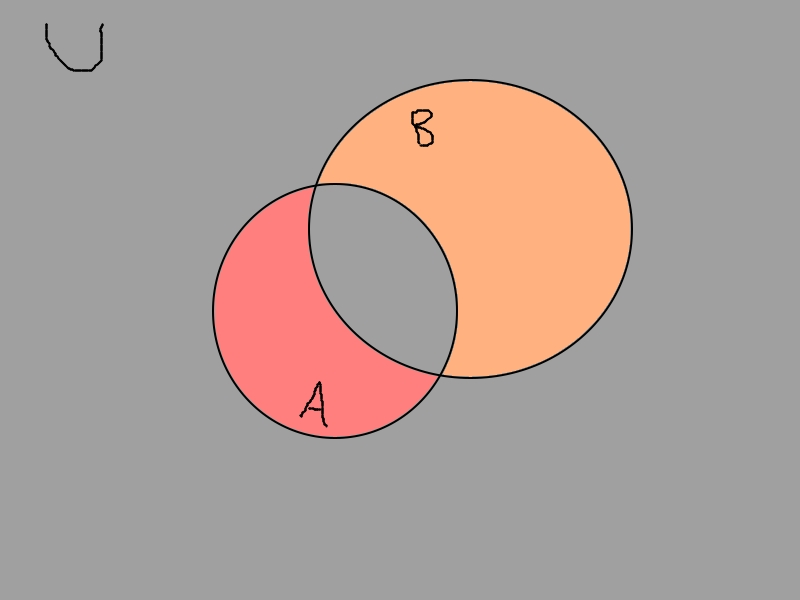
\includegraphics[scale=0.2]{venna.jpg}
\end{figure}
Із цього малюнку ми можемо вгадати тотожність:\\
$A \Delta B = (A \cup B) \setminus (A \cap B)$\\
Повторюю для себе: це - не доведення, а просто репрезентація
\end{example}

\subsection{Скінченні множини. Потужність}
Тут ми розглядаємо скінченні множини, тобто ті, що мають скінченну кількість елементім
\begin{definition}
\textbf{Потужністю} скінченної множини $A$ називають кількіть елементу множини $A$\\
Позначення: $|A| \overset{\text{або}}{=} n(A) \overset{\text{або}}{=} \text{card} A$
\end{definition}

\begin{example}
Скінченна множина $A = \{1,2,9\}$ має потужність \\ $n(A) = 3$
\end{example}

\begin{theorem}
Задані $A,B$ - скінченні множини, які не перетинаються\\
Тоді $n(A \cup B) = n(A) + n(B)$\\
\textit{Випливає з означення}
\end{theorem}

\begin{corollary}
Задані $A_1,\dots,A_n$ - скінченні множини, які попарно не перетинаються\\
Тоді $n(A_1 \cup \dots \cup A_n) = n(A_1) + \dots + n(A_n)$\\
\textit{Доводиться методом МІ}
\end{corollary}

\begin{theorem}
Задані $A,B$ - скінченні множини\\
Тоді $n(A \cup B) = n(A) + n(B) - n(A \cap B)$
\end{theorem}

\begin{pf}
Щоб довести формулу, нам треба використати формулу з \textbf{Crl. 2.5.4.}\\
Розглянемо три множини:\\
$D_1 = A \setminus B$ \hspace{1cm} $D_2 = A \cap B$ \hspace{1cm} $D_3 = B \setminus A$\\
Ці три множини попарно не перетинаються між собою. Тоді\\
$n(D_1 \cup D_2 \cup D_3) = n(D_1) + n(D_2) + n(D_3) = \\ = n(D_1) + n(D_2) + n(D_2) + n(D_3) - n(D_2) = n(D_1 \cup D_2) + n(D_2 \cup D_3) - n(D_2)$\\
$D_1 \cup D_2 \cup D_3 = A \cup B$\\
$D_1 \cup D_2 = A$\\
$D_2 \cup D_3 = B$\\
Таким чином, отримаємо:\\
$n(A \cup B) = n(A) + n(B) - n(A \cap B)$
\end{pf}
\bigskip \\
З'ясуємо тепер, а чому буде дорівнювати така формула при трьох множинах $A,B,C$\\
$n(A \cup B \cup C) = n(A \cup (B \cup C)) = n(A) + n(B \cup C) - n(A \cap (B \cup C) = \\ = n(A) + [n(B) + n(C) - n(B \cap C)] - n((A \cap B) \cup (A \cap C)) = \\ = n(A) + n(B) + n(C) - n(B \cap C) - [n(A \cap B) + n(A \cup C) - n((A \cap B) \cap (A \cap C))] = \\
=n(A)+n(B)+n(C) - n(A \cap B) - n(A \cap C) - n(B \cap C) + n(A \cap B \cap C)$\\
Тобто маємо, що спочатку ми беремо окремі множини, потім дві множини з усіма перетинами, а потім три множини з усіма перетинами. Причому знак змінюється: +,-,+
\bigskip \\
Можемо дану формулу узагальнити таким чином
\begin{corollary}
Задані $A_1,\dots,A_n$ - скінченні множини\\
Тоді $\huge n\left( A_1 \cup \dots \cup A_n \right) = \\ = \huge \sum_{1 \leq i \leq n} n(A_i) - \huge \sum_{1 \leq i < j \leq n} n(A_i \cap A_j) + \dots + (-1)^{n-1} n(A_1 \cap \dots \cap A_n)$\\
\textit{Це можна довести за МІ, але буде досить боляче}
\end{corollary}

\subsection{Декартів добуток}
\begin{definition}
\textbf{Декартовим добутком} множин $A,B$ називають таку множину
\begin{align*}
A \times B = \{(a,b): a \in A, b \in B\}
\end{align*}\\
Якщо працюємо з однією множиною, можемо писати так: $A \times A = A^2$
\end{definition}

\begin{example}
Задано $A = \{1,2,3\}$, $B = \{x,y\}$. Запишемо декартовий добуток\\
$A \times B = \{(1,x),(1,y),(2,x),(2,y),(3,x),(3,y)\}$\\
$B \times A = \{(x,1),(x,2),(x,3),(y,1),(y,2),(y,3)\}$
\end{example}

\begin{remark}
Із цього прикладу маємо, що $A \times B \neq B \times A$
\end{remark}

\begin{remark}
Обидва множини можуть будуть різної природи, а тому для кожної треба вводити універсальну множину\\
$A \subset U_1$ \hspace{1cm} $B \subset U_2$\\
Універсальна множина для декартового добутку: $U = U_1 \times U_2$
\end{remark}

\begin{theorem}
Задані $A,B$ - скінченні множини. Тоді\\
$n(A \times B) = n(A) \cdot n(B)$
\end{theorem}

\begin{pf}
Задамо $A = \{a_1,a_2,\dots,a_n\}$ \hspace{0.5cm} $B = \{b_1,b_2,\dots,b_m\}$\\
Розмістимо всі елементи множини $A \times B$ у вигляді такої таблиці\\
\begin{center}
\begin{tabular}{c|cccc}
$ $ & $b_1$ & $b_2$ & $\dots$ & $b_m$ \\
\hline
$a_1$ & $(a_1,b_1)$ & $(a_1,b_2)$ & $\dots$ & $(a_1,b_m)$ \\
$a_2$ & $(a_2,b_1)$ & $(a_2,b_2)$ & $\dots$ & $(a_2,b_m)$ \\
$\vdots$ & $\vdots$ & $\vdots$ & $\ddots$ & $\vdots$ \\
$a_n$ & $(a_n,b_1)$ & $(a_n,b_2)$ & $\dots$ & $(a_n,b_m)$
\end{tabular}
\end{center}
Зрозуміло, що така таблиця містить $n \cdot m = n(A) \cdot n(B)$ елементів\\
Тоді й маємо $n(A \times B) = n(A) \cdot n(B)$
\end{pf}

\begin{remark}
Можна визначити декартовий добуток для довільної скінченної кількості множин
\begin{align*}
A_1 \times \dots \times A_n = \{(a_1,\dots,a_n): a_1 \in A_1, \dots, a_n \in A_n\}
\end{align*}
Допустимо писати таким чином: $A \times \underset{n \text{ разів}}{\dots} \times A = A^n$\\
А також для скінченних множин $A_1,\dots,A_n$ справедлива рівність\\
$n(A_1 \times \dots \times A_n) = n(A_1) \cdots n(A_n)$\\
\textit{Доводиться завдяки МІ}
\end{remark}
Під час доведення деяких тотожностей з декартовим добутком зручно використовувати модельний метод
\begin{example}
Довести, що $A \times (B \cup C) = (A \times B) \cup (A \times C)$\\
$(x,y) \in A \times (B \cup C) \Leftrightarrow (x \in A) \wedge (y \in (B \cup C)) \Leftrightarrow \\ \Leftrightarrow (x \in A) \wedge ((y \in B) \vee (y \in C)) \Leftrightarrow ((x \in A) \wedge (y \in B)) \vee ((x \in A) \wedge (y \in C)) \\ \Leftrightarrow ((x,y) \in A \times B) \vee ((x,y) \in A \times C) \Leftrightarrow (x,y) \in (A \times B) \cup (A \times C)$
\end{example}
Також можемо використати аналог діаграми Венна, якщо є два множини. Перші компоненти множини - на осі ОХ; другі компоненти множини - на осі ОУ
\begin{figure}[H]
\centering
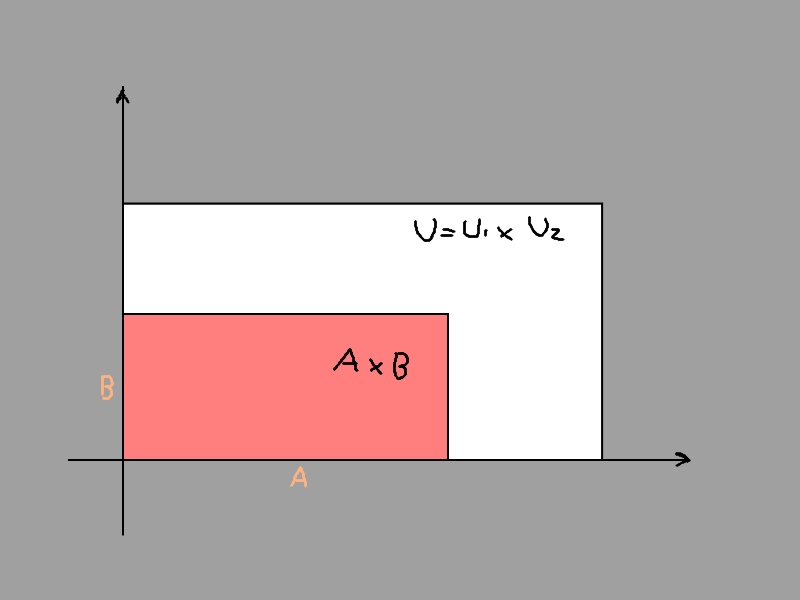
\includegraphics[scale=0.3]{venna2.jpg}
\end{figure}

\subsection{Розв'язок деяких рівнянь}
Розглянемо загальне рівняння вигляду
\begin{align*}
\mathcal{A}_1(X) = \mathcal{A}_2(X)
\end{align*}
Тут $\mathcal{A}_1, \mathcal{A}_2$ якісь формули алгебри множин, що містять скінченну кількість пропозиційних літер\\
$X$ - невідома множина, яку шукаємо\\
$\mathcal{A}_1(X) = \mathcal{A}_2(X)$\\
$\mathcal{A}_1(X) \Delta \mathcal{A}_2(X) = \emptyset$\\
Ліву частину рівності зобразимо в такому вигляді\\
$(\mathcal{B}_1 \cap X) \cup (\mathcal{B}_2 \cap \bar{X}) \cup \mathcal{B}_3 = \emptyset$\\
Тут $\mathcal{B}_i, i =1,2,3$ - якісь формули без невідомої $X$\\
Дане рівняння еквівалентне наступному\\
$\begin{cases}
\mathcal{B}_1 \cap X = \emptyset\\
\mathcal{B}_1 \cap \bar{X} = \emptyset\\
\mathcal{B}_3 = \emptyset\\
\end{cases}
 \iff 
 \begin{cases}
 X \subset \bar{\mathcal{B}_1} \\
 \mathcal{B}_2 \subset X \\
 \mathcal{B}_3 = \emptyset
 \end{cases} \iff 
 \begin{cases}
 \mathcal{B}_2 \subset X \subset \bar{\mathcal{B}_1} \\
 \mathcal{B}_3 = \emptyset
 \end{cases}$
 \\
 Відповідь: $\mathcal{B}_2 \subset X \subset \bar{\mathcal{B}_1}$ за умовою $\mathcal{B}_3 = \emptyset$. Інакше нема розв'язків
 
\begin{example}
Розв'язати рівняння $C \cup X = A \setminus B$\\
$C \cup X = A \setminus B$\\
$(C \cup X) \Delta (A \setminus B) = \emptyset$\\
$(C \cup X) \Delta (A \cap \bar{B}) = \emptyset$\\
$((C \cup X) \cap \overline{(A \cap \bar{B})}) \cup ((A \cap \bar{B}) \cap \overline{(C \cup X)}) = \emptyset$\\
$((C \cup X) \cap (\bar{A} \cup B)) \cup ((A \cap \bar{B} \cap \bar{C} \cap \bar{X}) = \emptyset$\\
$(C \cap \bar{A}) \cup (C \cap B) \cup (X \cap \bar{A}) \cup (X \cap B) \cup (\bar{X} \cap A \cap \bar{B} \cap \bar{C}) = \emptyset$\\
$\begin{cases}
(C \cap \bar{A}) \cup (C \cap B) = \emptyset \\
(X \cap \bar{A}) \cup (X \cap B) = \emptyset \\
\bar{X} \cap A \cap \bar{B} \cap \bar{C} = \emptyset
\end{cases} \iff
\begin{cases}
C \cap (\bar{A} \cup B) = \emptyset \\
(\bar{A} \cup B) \cap X = \emptyset \\
(A \cap \bar{B} \cap \bar{C}) \cap \bar{X} = \emptyset
\end{cases} \\
\iff
\begin{cases}
C \subset A \cap \bar{B} \\
X \subset A \cap \bar{B} \\
A \cap \bar{B} \cap \bar{C} \subset X
\end{cases} \iff
\begin{cases}
A \cap \bar{B} \cap \bar{C} \subset X \subset A \cap \bar{B} \\
C \subset A \cap \bar{B}
\end{cases} \\
\iff \begin{cases}
A \setminus (B \cup C) \subset X \subset A \setminus B \\
C \subset A \setminus B
\end{cases}$\\
Відповідь: $A \setminus (B \cup C) \subset X \subset A \setminus B$ за умовою $C \subset A \setminus B$. Інакше нема розв'язків
\end{example}

Буває випадки, коли треба розв'язати систему рівнянь
\begin{align*}
\begin{cases}
\mathcal{A}_1(X) = \mathcal{A}_2(X) \\
\mathcal{C}_1(X) = \mathcal{C}_2(X)
\end{cases}
\end{align*}
Ми просто розв'язуємо кожне рівняння окремо до останнього вигляду - а тому отримаємо такий вигляд\\
$\begin{cases}
 \mathcal{B}_2 \subset X \subset \bar{\mathcal{B}_1} \\
 \mathcal{B}_3 = \emptyset \\
  \mathcal{D}_2 \subset X \subset \bar{\mathcal{D}_1} \\
 \mathcal{D}_3 = \emptyset
\end{cases}
$\\
Перші два рівняння - розв'язок першого рівняння системи \\ Останні два рівняння - розв'язок другого рівняння системи\\
Тоді спрощується це рівняння ось таким чином \\
$\begin{cases}
\mathcal{B}_2 \cup \mathcal{D}_2 \subset X \subset \bar{\mathcal{B}_1} \cap \bar{\mathcal{D}_1} \\
\mathcal{B}_3 = \emptyset \\
\mathcal{D}_3 = \emptyset \\
\end{cases}$\\
Відповідь: $\mathcal{B}_2 \cup \mathcal{D}_2 \subset X \subset \bar{\mathcal{B}_1} \cap \bar{\mathcal{D}_1}$ за умовами $\mathcal{B}_3 = \emptyset$,
$\mathcal{D}_3 = \emptyset$. Інакше нема розв'язків\\
Останні дві умови можна суттєво спростити та переписати її в одну стрічку, якщо це буде можливо
\newpage

\section{Теорія відношень}
\subsection{Основа}
\begin{definition}
Задано $A_1,\dots,A_n$ - деякі множини\\
Множина $R$ називається \textbf{відношенням}, що задане на множинах $A_1,\dots,A_n$, якщо
\begin{align*}
R \subset A_1 \times \dots \times A_n
\end{align*}
$R = \emptyset$ - \textbf{порожнє відношення} \\
$R = A_1 \times \dots \times A_n$ - \textbf{повне відношення}
\end{definition}

\begin{example}
Задано $A_1 = \{1,2,3,4\}$, $A_2 = \{a,b,c,d\}$. Задамо відношення\\
$R = \{(1,a), (2,b), (2,c), (3,a), (4,b), (1,d) \}$
\end{example}

\textbf{Домовленість із позначеннями}\\
$R \subset A \times B \iff R: A \to B$\\
$(x,y) \in R \iff xRy$

\begin{example}
Із попереднього прикладу маємо відношення $R \subset A_1 \times A_2$, тобто $R: A_1 \to A_2$\\
Маємо $(1,a) \in R$, тобто $1Ra$
\end{example}

\begin{definition}
\textbf{Тотожнім відношенням} на множині $A$ називають таке відношення
\begin{align*}
I_A = \{(x,x): x \in A\}
\end{align*}
Тобто маємо, що $xI_A y \iff x = y$
\end{definition}

\textbf{Способи задання бінарних відношень}\\
1. Як стандартну множину: \\ $R = \{(1,a), (2,b), (2,c), (3,a), (4,b), (1,d)\}$\\
2. На координатній площині: \\
$R: \mathbb{R} \to \mathbb{R}$ \hspace{0.5cm} $R = \{(x,y): x^2+y^2 = 1 \}$\\
(INSERT PICTURE)\\
3. Стрілковими діаграмами: \\
$A = \{a_1,a_2,a_3\}$, $B = \{b_1,b_2\}$ \hspace{0.5cm} $R: A \to B$ \hspace{0.5cm} $R = \{(a_1,b_1), (a_2,b_2), (a_3,b_1)\}$\\
(INSERT PICTURE)\\
4. Матрицею \\
$R = \{(a_1,b_1), (a_2,b_2), (a_3,b_1)\}$\\
$M_{R} = \begin{pmatrix}
1 & 0 \\
0 & 1 \\
1 & 0
\end{pmatrix}$\\
5. На графах\\
$A = \{a,b,c\}$ \hspace{0.5cm} $R: A \to A$ \hspace{0.5cm} $R = \{(a,b), (b,c), (c,c)\}$\\
(INSERT PICTURE)
\bigskip \\
Перший спосіб не обов'язково для бінарних. П'ятий спосіб бінарне відношення задається лише на одній множині

\subsection{Основні операції}
\begin{definition}
Задано відношення $R,S \subset A_1 \times \dots \times A_n$\\
\textbf{Об'єднанням} відношень $R,S$ називають об'єднання множин $R \cup S$\\
\textbf{Перетином} відношень $R,S$ називають об'єднання множин $R \cap S$\\
\textbf{Доповненням} відношення $R$ називають доповненням множин $\bar{R}$ відносно універсальної множини $U = A_1 \times \dots \times A_n$
\end{definition}

\begin{definition}
Задано відношення $R: A \to B$, $S: B \to C$ \\
\textbf{Інверсним} відношенням називають відношення $R^{-1}: B \to A$, для якого
\begin{align*}
bR^{-1}a \iff aRb
\end{align*}
\textbf{Композицією} відношень називають відношення $R \circ S: A \to C$, для якого
\begin{align*}
a(R \circ S)c \iff \exists b: aRb \wedge bSc
\end{align*}
\end{definition}

\begin{remark}
Задано відношення $R: A \to B$, $S: A \to B$, де $A,B$ - скінченні множини \\
Тоді ми маємо матриці $M_R, M_S$\\
Щоб отримати $M_{R \cup S}$, треба поелементно провести диз'юнкцію, тобто \\ $(M_{R \cup S})_{ij} = (M_R)_{ij} \vee (M_S)_{ij}$\\
Щоб отримати $M_{R \cap S}$, треба поелементно провести кон'юнкцію, тобто \\ $(M_{R \cap S})_{ij} = (M_R)_{ij} \wedge (M_S)_{ij}$\\
Щоб отримати $M_{\bar{R}}$, треба від кожного елементу взяти заперечення, тобто \\ $(M_{\bar{R}})_{ij} = \neg (M_R)_{ij}$\\
Щоб отримати $M_{R^{-1}}$, треба транспонувати матрицю, тобто \\ $M_{R^{-1}} = M_R^T$\\
Щоб отримати $M_{R \circ S}$, якщо $S: B \to C$, треба перемножити обидві матриці, тобто \\ $M_{R \circ S} = M_R M_S$
\end{remark}

\begin{example}
(INSERT EXAMPLE)
\end{example}

\begin{theorem}
$R \circ (S \circ T) = (R \circ S) \circ T$
\end{theorem}

\begin{pf}
$a (R \circ (S \circ T))d \iff \exists b: aRb \wedge b(S \circ T)d \iff \exists b: aRb \wedge (\exists c: bSc \wedge cTd) \\ \iff \exists b \exists c: aRb \wedge bSc \wedge sTd \iff \exists c: (\exists b: aRb \wedge bSc) \wedge sTd \\ \iff \exists c: a(R \circ S)c \wedge sTd \iff a((R \circ S) \circ T)d$
\end{pf}

\subsection{Властивості бінарних відношень}
\begin{definition}
Задано відношення $R: A \to A$\\
Відношення називається \textbf{рефлексивним}, якщо
\begin{align*}
\forall a \in A: aRa
\end{align*}
Відношення називається \textbf{антирефлексивним}, якщо
\begin{align*}
\forall a \in A:  \neg aRa
\end{align*}
Відношення називається \textbf{симетричним}, якщо
\begin{align*}
a_1 R a_2 \iff a_2 R a_1
\end{align*}
Відношення називається \textbf{антисиметричним}, якщо
\begin{align*}
a_1 R a_2 \wedge a_2 R a_1 \implies a_1 = a_2
\end{align*}
Відношення називається \textbf{транзитивним}, якщо
\begin{align*}
a_1 R a_2 \wedge a_2 R a_3 \implies a_1 R a_3
\end{align*}
\end{definition}

\begin{example}
Дослідимо ось таке відношення $R: A \to A$, де $A = \{1,2,3,4\}$ на властивості\\
$R = \{(1,1),(1,4),(2,1),(2,2),(3,1),(3,2),(4,4)\}$\\
- не рефлексивне, тому що $\exists 3 \in A: \neg 3R3$\\
- не антирефлексивне, тому що $\exists 1 \in A: 1R1$\\
- не симетричне, тому що $1R4 \not\Leftrightarrow 4R1$\\
- антисиметричне, тому що кожна симетрична пара чисел дає нам пару однакових чисел\\
- не транзитивне, тому що $2R1 \wedge 1R4 \not\Rightarrow 2R4$
\end{example}

\begin{remark}
Порожнє відношення $\emptyset$ є рефлексивним, антирефлексивнми, симетричнми, антисиметричним, транзитивним. Просто тому що нема жодної пари точок, які б порушили всі п'ять означень
\end{remark}

\begin{proposition}
Задано відношення $R: A \to A$\\
$R$ - рефлексивне $\iff R \supset I_A$\\
$R$ - антирефлексивне $\iff R \cap I_A = \emptyset$\\
$R$ - симетричне $\iff R = R^{-1}$\\
$R$ - антисиметричне $\iff R \cap R^{-1} \subset I_A$\\
$R$ - транзитивне $\iff R \circ R \subset R$\\
\end{proposition}

\begin{pf}
\rightproof Дано: $R$ - рефлексивне\\
$\forall a \in A: aI_Aa \overset{\text{умова}}{\Rightarrow} aRa$. Отже, $I_A \subset R$\\
\leftproof Дано: $R \supset I_A$\\
$\forall a \in A: aI_Aa \overset{\text{умова}}{\Rightarrow} aRa$. Отже, $R$ - рефлексивне
\bigskip \\
\rightproof Дано: $R$ - антирефлексивне, тобто $\forall a \in A: \neg aRa$\\
Водночас $I_A = \{(a,a), a \in A \}$.
Отже, $R \cap I_A = \emptyset$\\
\leftproof Дано: $R \cap I_A = \emptyset$\\
$\forall a \in A: aI_Aa$, тоді за умовою, $\neg aRa$, інашке перетин двох множин був би не порожнім.
Отже, $R$ - антирефлексивне
\bigskip \\
$R$ - симетричне $\iff$
$(a_1 R a_2 \iff a_2 R a_1 \iff a_1 R^{-1} a_2) \iff R = R^{-1}$
\bigskip \\
\rightproof Дано: $R$ - антисиметричне, тобто $a_1 R a_2 \wedge a_2 R a_1 \implies a_1 = a_2$\\
$x(R \cap R^{-1})y \Rightarrow xRy \wedge xR^{-1}y \Rightarrow xRy \wedge yRx \Rightarrow x=y$\\
Тоді $x(R \cap R^{-1})x \Rightarrow xI_Ax$. Отже, $R \cap R^{-1} \subset I_A$\\
\leftproof Дано: $R \cap R^{-1} \subset I_A$\\
$xRy \wedge yRx \Rightarrow xRy \wedge xR^{-1}y \Rightarrow x(R \cap R^{-1})y \Rightarrow xI_Ay \Rightarrow x = y$.
Отже, $R$ - антисиметричне
\bigskip \\
\rightproof Дано: $R$ - транзитивне, тобто $a_1 R a_2 \wedge a_2 R a_3 \implies a_1 R a_3$\\
$x(R \circ R)z \Rightarrow \exists y: xRy \wedge yRz \Rightarrow xRz$. Отже, $R \circ R \subset R$\\
\leftproof Дано: $R \circ R \subset R$\\
$a_1 R a_2 \wedge a_2 R a_3 \Rightarrow a_1 (R \circ R) a_3 \Rightarrow a_1 R a_3$. Отже, $R$ - транзитивне
\end{pf}

\subsection{Транзитивне замикання}
\begin{definition}
Задано відношення $R, R^+: A \to A$\\
Відношення $R^+$ називають \textbf{транзитивним замиканням} відношення $R$, якщо
\begin{align*}
R \subset R^+ \\
R^+ - \text{найменше транзитивне відношення}
\end{align*}
\end{definition}

\begin{example}
Маємо відношення \\ $R = \{(1,1),(1,4),(2,1),(2,2),(3,1),(3,2),(4,4)\}$\\
Транзитивним замиканням відношення $R$ буде таке відношенння\\
$R^+ = \{(1,1),(1,4),(2,1),(2,2),(3,1),(3,2),(4,4),(2,4),(3,4)\}$\\
$R \subset R^+$, а також $R^+$ - найменше транзитивне відношення. Інакше якщо добавити інші точки, то або ми нічого не згенеруємо, або отримаємо нові пари задля збереження транзитивності
\end{example}

\begin{remark}
Транзитивне замикання задається однозначно\\
Дійсно, маємо $R_1^+, R_2^+$. Тоді вони обидва найменші транзитивні, або математично записуючи\\
$\forall S \text{ - транзитивне}: S \supset R \Rightarrow S \supset R^+$\\
Для $R_1^+$ маємо, що $R_1^+ \supset R \Rightarrow R_1^+ \supset R_2^+$\\
Для $R_1^+$ маємо, що $R_2^+ \supset R \Rightarrow R_2^+ \supset R_1^+$\\
Отже, $R_1^+ = R_2^+$
\end{remark}

\begin{proposition}
$R^+ = \huge \bigcup_{n=1}^\infty R^n$\\
\textit{Поки без доведення}
\end{proposition}

\begin{theorem}
Задано $A$ - така множина, що $n(A) = N$. Тоді\\
$R^+ = \huge \bigcup_{n=1}^N R^n$\\
\textit{Поки без доведення}
\end{theorem}

\begin{example}
Задано $A = \mathbb{N}$ та відношення $R = \{(n,n+1): n \in \mathbb{N}\}$. Знайдемо його транзитивне замикання\\
Використовуючи метод МІ, можемо показати, що\\
$\forall k \geq 1: R^k = \{(n,n+k): n \in \mathbb{N}\}$\\
$\Rightarrow R^+ = \huge \bigcup_{k=1}^\infty R^k = \\ = \{(n,n+1), k =1, n \in \mathbb{N}\} \cup \{(n,n+2), k =2, n \in \mathbb{N}\} \cup \dots = \\
= \{(n,n+k): n \in \mathbb{N}, k \in \mathbb{N}\} \overset{\text{або}}{=} \{(n,k): n < k\}$
\end{example}

\begin{example}
Задано $A = \{a,b\}$ та відношення $R = \{(a,b),(b,a)\}$. Знайдемо його транзитивне замикання\\
Оскільки $n(A) = 2$, то тоді $R^+ = R \cup R^2$\\
$R^2 = \{(a,a),(b,b)\}$\\
$\Rightarrow R^+ = \{(a,a),(a,b),(b,a),(b,b)\} = A^2$
\end{example}

\subsection{Відношення еквівалентності}
\begin{definition}
Задано відношення $R: A \to A$\\
Його називають \textbf{відношенням еквівалентності}, якщо $R$ - рефлексивне, симетричне, транзитивне одночасно\\
Позначення: $xRy \iff x \sim y$
\end{definition}

\begin{example}
Задано $A = \mathbb{Z}, p \in \mathbb{N}$. Встановимо таке відношення $R$:\\
$x \sim y \iff (x-y) \text{ mod } p = 0$\\
Це відношення - дійсно еквівалентне, оскільки:\\
- $(x-x) \text{ mod } p = 0 \text{ mod } p = 0$\\
- $(x-y) \text{ mod } p = 0 \iff -(y-x) \text{ mod } p = 0 \iff (y-x) \text{ mod } p = 0$\\
- $(x-y) \text{ mod } p = 0$ та $(y-z) \text{ mod } p = 0$ \\ Тоді $(x-z) \text{ mod } p = (x-y+y-z) \text{ mod } p = (x-y) \text{ mod } + (y-z) \text{ mod } = 0$\\
Отже, можемо ми мати такий ланцюг еквівалентності:\\
$1 \sim p+1 \sim -2p+1$ \hspace{1cm} $0 \sim 10p$\\
Проте $1 \not\sim 2$
\end{example}

\begin{example}
Задано $A = \{1,2,3,4,5,6\}$ та відношення\\
$R = \{(1,1),(2,2),(3,3),(4,4),(5,5),(6,6),(1,2),(2,1),(3,4),(4,3),(3,5), \\ (5,3),(4,5),(5,4)\}$\\
Це відношення (перевірити самостійно) рефлексивне, симетричне, транзитивне - отже, еквівалентне\\
Тоді $1 \sim 2$ \hspace{0.5cm} $3 \sim 4 \sim 5$ \hspace{0.5cm} $6$\\
Проте $1 \not\sim 3$ \hspace{0.5cm} $1 \not\sim 6$ \hspace{0.5cm} $3 \not\sim 6$
\bigskip \\
До речі, представимо відношення у вигляді матриці\\
$M_{\sim} = \begin{pmatrix}
1 & 1 & 0 & 0 & 0 & 0 \\
1 & 1 & 0 & 0 & 0 & 0 \\
0 & 0 & 1 & 1 & 1 & 0 \\
0 & 0 & 1 & 1 & 1 & 0 \\
0 & 0 & 1 & 1 & 1 & 0 \\
0 & 0 & 0 & 0 & 0 & 1 \\
\end{pmatrix}$\\
Мажмо такі блокові матриці з одиниць, $2 \times 2$, $3 \times 3$ та $1 \times 1$
\end{example}

\subsection{Відношення порядку}
\begin{definition}
Задано відношення $R: A \to A$\\
Його називають \textbf{відношенням еквівалентності}, якщо $R$ - рефлексивне, антисиметричне, транзитивне одночасно\\
Множина $A$ тоді називається \textbf{частково впорядкованою}\\
Позначення: $x \preceq y \iff xRy$
\end{definition}

\begin{remark}
Деякі зауваження стосовно передування:\\
$s \succeq  y \iff y \preceq x$\\
$x \succ y \iff y \prec x \iff (y \preceq x) \wedge (x \neq y)$
\end{remark}

\begin{example}
Задано $A = \mathbb{R}$. Відошення $xRy \iff x \leq y$ - відношення порядку, тому що\\
- $x \leq x$ \\
- $(x \leq y) \wedge (y \leq x) \Rightarrow x = y$ \\
- $(x \leq y) \wedge (y \leq z) \Rightarrow x \leq z$\\
Тоді
$x \preceq y \iff x \leq y$
\end{example}

\begin{definition}
Якщо $(x \preceq y) \vee (y \preceq x)$, тоді $x,y$ називають \textbf{порівняльними}\\
Якщо порівняльні $\forall x,y$, то тоді маємо \textbf{відношення лінійного порядку}
\end{definition}

\subsection{Розбиття множин, фактор-множини}
\begin{definition}
Задано $U \neq \emptyset$ - деяка універсальна множина\\
Сукупність множин $\{A_{\alpha}: \alpha \in I\}$ назвемо \textbf{розбиттям} множини $U$, якщо
\begin{align*}
\forall \alpha \in I: A_\alpha \neq \emptyset\\
U = \huge\bigcup_{\alpha \in I} A_\alpha\\
\forall \alpha_1 \neq \alpha_2: A_{\alpha_1} \cap A_{\alpha_2} = \emptyset
\end{align*}
\end{definition}

\begin{example}
Нехай $U = \{1,2,3,4,5\}$\\
$U = \underset{A_1}{\{1,2\}} \cup \underset{A_2}{\{3,5\}} \cup \underset{A_3}{\{4\}}$\\
Множини $A_1,A_2,A_3$ не перетинаються попарно\\
Таким чином, маємо розбиття $\{\underset{A_1}{\{1,2\}}, \underset{A_2}{\{3,5\}}, \underset{A_3}{\{4\}} \}$
\end{example}

\begin{example}
Нехай $U = \mathbb{R}^2$. Задамо такі множини:\\
$A_r = \{(x,y): x^2+y^2 = r^2\}$, де $r \geq 0$\\
Множина $\{A_r, r \geq 0\}$ утворює розбиття множини $\mathbb{R}^2$\\
(INSERT PICTURE)
\end{example}

\begin{definition}
Задано відношення еківалентності $R$ на множині $A$. Нехай $a \in A$\\
\textbf{Класом еквівалетності}, породженим елементом $a$, називають таку множину
\begin{align*}
[a] = \{x \in A: x \sim a\}
\end{align*}
\end{definition}

\begin{remark}
$[a] \neq \emptyset$, принаймні тому що $a \in A$
\end{remark}

\begin{example}
Повернімось до $A = \{1,2,3,4,5,6\}$ та відношення\\
$R = \{(1,1),(2,2),(3,3),(4,4),(5,5),(6,6),(1,2),(2,1),(3,4),(4,3),(3,5), \\ (5,3),(4,5),(5,4)\}$\\
З'ясовано, що $1 \sim 2$ \hspace{0.5cm} $3 \sim 4 \sim 5$ \hspace{0.5cm} $6$\\
Маємо тоді такі класи еквівалентності\\
$[1] = [2] = \{1,2\}$ \hspace{0.5cm} $[3] = [4] = [5] = \{3,4,5\}$ \hspace{0.5cm} $[6] = \{6\}$\\
Можемо вже зауважити, що або класи еквівалетності співпадають, або не перетинаються взагалі. Чи буде це завжди?
\end{example}

\begin{theorem}
Класи еквівалентності не перетинаються або співпадають
\end{theorem}

\begin{pf}
Тобто доводимо, що $\forall a_1 \in a_2 \in A: ([a_1] \cap [a_2] = \emptyset) \vee ([a_1] = [a_2])$\\
Розглянемо деякий елемент $b \in [a_1] \cap [a_2] \neq \emptyset$\\
$b \in [a_1] \Rightarrow b \sim a_1$\\
$b \in [a_2] \Rightarrow b \sim a_2$\\
$(a_1 \sim b) \wedge (b \sim a_2) \Rightarrow (a_1 \sim a_2)$\\
Лишилось довести, що $[a_1] = [a_2]$\\
$x \in [a_1] \iff x \sim a_1 \iff x \sim a_2 \iff x \in [a_2]$
\end{pf}

\begin{definition}
Задано відношення еківалентності $R$ на множині $A$ \\
\textbf{Фактор-множиною} множини $A$ називають таку множину
\begin{align*}
A/_{\sim} = \{[a]: a \in A\}
\end{align*}
\end{definition}

\begin{example}
Профакторизуємо множину $A = \{1,2,3,4,5,6\}$ за попереднім відношенням еквівалетності\\
$1 \sim 2$ \hspace{0.5cm} $3 \sim 4 \sim 5$ \hspace{0.5cm} $6$\\
$A/_{\sim} = \{[1],[3],[6]\} = \{\{1,2\}, \{3,4,5\}, \{6 \} \}$
\end{example}

\begin{example}
Профакторизуємо множину $\mathbb{Z}$ за відношенням еквівалентності\\
$x \sim y \iff (x-y) \text{ mod } p = 0$\\
При діленні на $p$ маємо такі остачі: $0,1,\dots,p-1$\\
Тому маємо такі класи еквівалентності:\\
$[0] = \{\dots, -2p, -p, 0, p, 2p, \dots\} = \{0 + jp, j \in \mathbb{Z}\}$\\
$[1] = \{\dots, -2p+1, -p+1, 1, p+1, 2p+1, \dots\} = \{1 + jp, j \in \mathbb{Z}\}$\\
$\dots$\\
$[p-1] = \{\dots, -p-1, -1, p-1, 2p-1, 3p-1, \dots\} = \{p-1 + jp, j \in \mathbb{Z}\}$\\
Коротше кажучи, $\forall k: 0 \leq k \leq p-1: A_k = [k] = \{k+jp, j \in \mathbb{Z}\}$\\
Запишемо фактор-множину\\
$A/_{\text{mod } p} = \{A_k: 0 \leq k \leq p-1\}$
\end{example}

\subsection{Функція як окремий випадок відношення}
Тут вивчається зв'язок між бінарними відношеннями та функціями з матану
\begin{definition} 
Задано відношення $R: A \to B$\\
\textbf{Областю визначення} відношення $R$ назвемо множину
\begin{align*}
\mathcal{D}_R = \{x \in A: \exists y \in B: xRy\}
\end{align*}
\textbf{Областю значень} (або \textbf{образом}) відношення $R$ назвемо множину
\begin{align*}
\Im_R = \{y \in B: \exists x \in A: xRy\}
\end{align*}
\end{definition}

\begin{proposition}
$\mathcal{D}_R = \Im_{R^{-1}}$\\
\textit{Вправа: довести}
\end{proposition}

\begin{definition}
Задано відношення $R: A \to B$\\
Відношення $R$ називається \textbf{сюр'єктивним}, якщо
\begin{align*}
\forall y \in B: \exists x \in A: xRy
\end{align*}
Відношення $R$ називається \textbf{ін'єктивним}, якщо
\begin{align*}
(x_1Ry) \wedge (x_2Ry) \Rightarrow x_1 = x_2
\end{align*}
\end{definition}

\begin{proposition}
$R$ - сюр'єктивне $\iff \Im_R = B$\\
\textit{Вправа: довести}
\end{proposition}

\begin{definition}
Задано відношення $R: A \to B$\\
Відношення $R$ називається \textbf{функціональним}, якщо
\begin{align*}
(xRy_1) \wedge (xRy_2) \Rightarrow y_1 = y_2
\end{align*}
Саме звідси виникають функції як в класичному матані. Кожному $x$ ставиться у відповідніть єдине $y$\\
Вважатимемо надалі, що функціональному відношенню $R_f: A \to B$ відповідає функція $f: A \to B$, така, що
\begin{align*}
\mathcal{D}_f = \mathcal{D}_{R_f} \\
y = f(x) \iff xR_fy
\end{align*}
\end{definition}


\begin{proposition}
$R$ - ін'єктивне $\iff R^{-1}$ - функціональне\\
\textit{Вправа: довести}
\end{proposition}

\begin{theorem}
Задані відношення $R: A \to B$, $S: B \to C$\\
$R,S$ - сюр'єктивні. Тоді $R \circ S$ - сюр'єктивне\\
$R,S$ - ін'єктивні. Тоді $R \circ S$ - ін'єктивне\\
$R,S$ - функціональні. Тоді $R \circ S$ - функціональне
\end{theorem}

\begin{pf}
$R,S$ - сюр'єктивні\\
Нехай $z \in C$. Тоді за сюр'єктивністю $S$, $\exists y \in B: ySz$\\
Тоді за сюр'єктивністю $R$, $\exists x \in A: xRy$\\
Тобто $\forall z \in C: \exists x \in A: x(R \circ S)z$. Отже, $R \circ S$ - сюр'єктивне
\bigskip \\
$R,S$ - ін'єктивні\\
Нехай $x_1(R \circ S)z, x_2(R \circ S)z$. За означенням,\\
$\exists y_1,y_2 \in B: x_1Ry_1, x_2Ry_2, y_1Sz, y_2Sz$\\
За ін'єктивністю $S$, $y_1 = y_2 = y$. Отже, $x_1Ry,x_2Ry$\\
За ін'єктивністю $R$, $x_1 = x_2$. Отже, $R \circ S$ - ін'єктивне
\bigskip \\
$R,S$ - функціональні\\
\textit{Вправа: довести}
\end{pf}

\begin{definition}
Функцію $f: A \to B$ називають \textbf{відображенням}, якщо
\begin{align*}
\forall x \in A: \mathcal{D}_f = A
\end{align*}
\end{definition}

\begin{proposition}
Задано $R_f$ - функціональне відображення\\
$f$ - відображення $\iff (R_f)^{-1}$ - сюр'єктивне
\end{proposition}

\begin{proposition}
Задані функції $f: A \to B$, $g: B \to C$ - відображення\\
Тоді $g \circ f$ - відображення
\end{proposition}

\begin{definition} Маємо відображення \\
\textbf{Ін'єкцією} називають відображення, що відповідає ін'єктивному \\ функціональному відношенню\\
\textbf{Сюр'єкцією} називають відображення, що відповідає сюр'єктивному \\ функціональному відношенню\\
\textbf{Бієкцією} називають відображення, що є ін'єкцією та сюр'єкцією одночасно\\
\end{definition}
\newpage
\end{document}